\documentclass[11pt]{article}
\usepackage{amssymb, amsmath, libertine, hyperref, xcolor, booktabs, enumitem, microtype}
\usepackage[T1]{fontenc}
\usepackage[margin=1in]{geometry}
\usepackage{tikz}
\newcommand{\gridxy}[4]{% xmin xmax ymin ymax -- gridlines exactly on the ticks
  \foreach \gX in {#1,...,#2} \draw[gray!25] (\gX,#3) -- (\gX,#4);
  \foreach \gY in {#3,...,#4} \draw[gray!25] (#1,\gY) -- (#2,\gY);}
\definecolor{dark-red}{rgb}{0.4,0.15,0.15}
\definecolor{blue-g}{rgb}{0.15,0.28,0.45}
\hypersetup{colorlinks, linkcolor=dark-red, urlcolor=dark-red}
\setlist[enumerate,1]{label=(\alph*), leftmargin=*, itemsep=5pt, topsep=5pt}
\setlist[enumerate,2]{label=(\roman*), leftmargin=*, itemsep=2pt, topsep=2pt}
\pagestyle{empty}
\newcommand{\prob}[2]{\medskip\noindent\textbf{\large #1}\hfill\textit{#2}\par\smallskip}
\begin{document}

\begin{center}
{\Large\bfseries Math 111: Calculus \quad Practice Exam 3}\\[4pt]
{For Exam 3, in class on Friday, November 20}
\end{center}

\medskip
\noindent\textbf{What Exam 3 is like.} Four problems in a fifty-minute period, closed-book
and device-free. It is \textbf{cumulative}: the new material is accumulation and the
definite integral (\S4.1--\S4.3), numerical integration (\S5.6), and both Fundamental
Theorems (\S4.4, \S5.1, \S5.2), but earlier ideas --- reading a graph, over- and
under-estimates, the tangent line, the chain rule, critical numbers --- come back inside the
new problems. Substitution (\S5.3, Monday the 16th) is \emph{not} on Exam~3. Each problem is
marked holistically on the 0--5 scale: a right answer with no reasoning is not a 5, and a
wrong answer containing a real idea is not a 0.

\smallskip
\noindent\textbf{How to use this.} Sit down with a blank sheet and fifty minutes on a
clock, book closed and phone in another room. Bring whatever you could not finish to
review on Wednesday the 18th.

\smallskip
\noindent\textbf{Reference sheet.} The last page is a reference sheet of antiderivatives and
integral rules. I am providing it: the same sheet will be the last page of Exam~3, and you
may use it there. Practice with it now.

\bigskip\hrule

\prob{1. Rain, from a rate}{about 12 minutes}
During a storm, the rate at which rain fell, $r(t)$ in millimeters per hour, was
recorded every hour:
\smallskip
\begin{center}
\begin{tabular}{@{}lrrrrr@{}}
\toprule
$t$ (hours) & 0 & 1 & 2 & 3 & 4\\
$r(t)$ (mm/hr) & 0 & 2 & 5 & 9 & 14\\
\bottomrule
\end{tabular}
\end{center}
\smallskip
Assume $r$ is increasing on $[0,4]$.
\begin{enumerate}
\item In a sentence, with units, say what $\int_0^4 r(t)\,dt$ means.
\item Compute $L_4$ and $R_4$, with units. Which is an over-estimate and which an
under-estimate of $\int_0^4 r(t)\,dt$? Explain with a picture, not a rule.
\item Compute the trapezoid estimate $T_4$. The differences in the table suggest $r$ is
concave up; assuming it is, is $T_4$ too large or too small? Explain with a picture of a
single subinterval.
\item Use the readings at $t=1$ and $t=3$ to compute the midpoint estimate $M_2$. Assuming
$r$ is concave up, is it too large or too small? Combine your answers to (c) and (d) into
an interval that must contain the true total rainfall.
\end{enumerate}

\prob{2. Accumulating a graph}{about 14 minutes}
The graph of $f$ on $[0,8]$ is below; it is made of straight segments. Let
\[A(x)=\int_0^xf(t)\,dt\qquad\text{for }0\le x\le8.\]
\begin{center}
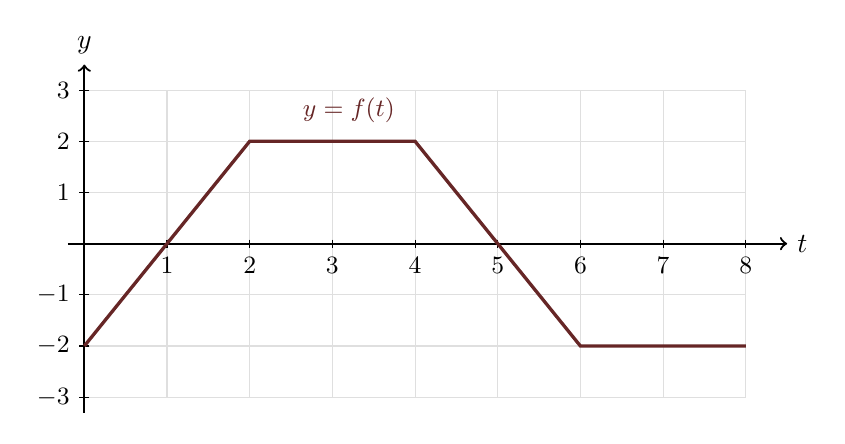
\begin{tikzpicture}[x=1.05cm,y=0.65cm]
  \gridxy{0}{8}{-3}{3}
  \draw[->,thick] (-0.2,0) -- (8.5,0) node[right] {$t$};
  \draw[->,thick] (0,-3.3) -- (0,3.5) node[above] {$y$};
  \foreach \x in {1,...,8} \draw (\x,0.08) -- (\x,-0.08) node[below,font=\small] {\x};
  \foreach \y in {-3,-2,-1,1,2,3} \draw (0.06,\y) -- (-0.06,\y) node[left,font=\small] {$\y$};
  \draw[very thick, dark-red] (0,-2) -- (2,2) -- (4,2) -- (6,-2) -- (8,-2);
  \node[dark-red,font=\small] at (3.2,2.6) {$y=f(t)$};
\end{tikzpicture}
\end{center}
\begin{enumerate}
\item Find $A(1)$, $A(2)$, $A(5)$ and $A(8)$.
\item On which intervals is $A$ increasing, and on which decreasing? Find every local maximum
and local minimum of $A$ in $(0,8)$, and the global maximum and minimum of $A$ on $[0,8]$.
\item Find $A'(3)$ and $A'(7)$, and say which theorem you are using. Where is $A$ concave up,
concave down, and straight?
\item A classmate writes: ``$A'(x)=f(x)$, and the largest value of $f$ on $[0,8]$ is $2$,
which $f$ first reaches at $x=2$. So $A$ has its maximum at $x=2$.'' Find the first wrong
step, say why it is wrong, and say where $A$ does have its maximum.
\end{enumerate}

\prob{3. Evaluating with the FTC}{about 12 minutes}
Use the Fundamental Theorem of Calculus. Show the antiderivative you use, and check it
by differentiating.
\begin{enumerate}
\item $\displaystyle\int_1^4\Big(3\sqrt x-\frac2{x^2}\Big)\,dx$
\item $\displaystyle\int_0^{\pi/2}\cos x\,dx$, and say in a sentence what this number means
in terms of a graph.
\item The average value of $\sin x$ on $[0,\pi]$.
\item A classmate writes: ``An antiderivative of $\frac1x$ is $\ln|x|$, so
$\int_{-1}^{2}\frac1x\,dx=\ln|2|-\ln|-1|=\ln2$.'' Is this right? Find the first wrong
step, and say what hypothesis of the theorem is involved.
\end{enumerate}

\prob{4. Differentiating accumulations}{about 12 minutes}

\begin{enumerate}
\item Find each derivative, and say which rule or theorem you use.
\begin{enumerate}
\item $\displaystyle\frac{d}{dx}\int_2^x\sin(t^2)\,dt$
\item $\displaystyle\frac{d}{dx}\int_x^5\sqrt{1+t^4}\,dt$
\item $\displaystyle\frac{d}{dx}\int_0^{x^3}e^{-t^2}\,dt$
\end{enumerate}
\item Let $G(x)=\int_0^x(t^2-3t)\,dt$. Without finding a formula for $G$, find the critical
numbers of $G$ and classify each as a local maximum, local minimum, or neither.
\item Let $A(x)=\int_1^x\sqrt{t^3+1}\,dt$. Find the tangent line to $A$ at $x=1$ and use it to
estimate $A(1.1)$. Is your estimate too large or too small? Explain.
\end{enumerate}

\newpage
\begin{center}
{\Large\bfseries Reference sheet: antiderivatives and integrals}\\[4pt]
\fcolorbox{dark-red}{white}{\parbox{0.9\textwidth}{\centering\small
\textbf{Provided by your instructor for Exam~3.} It is attached to the exam, and you may use anything on it.\\
You do not need to memorize what is here; you do need to know when and why to use it.}}
\end{center}

\noindent\textbf{Basic antiderivatives.} Each line is a derivative fact read backwards.
Check any antiderivative by differentiating it.

\smallskip
\begin{center}
\renewcommand{\arraystretch}{1.95}
\begin{tabular}{@{}l@{\qquad}l@{\qquad}l@{}}
\toprule
\textbf{derivative fact} & \textbf{antiderivative} & \textbf{note}\\
\midrule
$\dfrac{d}{dx}\dfrac{x^{n+1}}{n+1}=x^n$ & $\displaystyle\int x^n\,dx=\frac{x^{n+1}}{n+1}+C$ & $n\neq-1$\\
$\dfrac{d}{dx}\ln|x|=\dfrac1x$ & $\displaystyle\int\frac1x\,dx=\ln|x|+C$ & the $n=-1$ case\\
$\dfrac{d}{dx}e^x=e^x$ & $\displaystyle\int e^x\,dx=e^x+C$ & \\
$\dfrac{d}{dx}a^x=a^x\ln a$ & $\displaystyle\int a^x\,dx=\frac{a^x}{\ln a}+C$ & $a>0$, $a\neq1$\\
$\dfrac{d}{dx}(-\cos x)=\sin x$ & $\displaystyle\int\sin x\,dx=-\cos x+C$ & \\
$\dfrac{d}{dx}\sin x=\cos x$ & $\displaystyle\int\cos x\,dx=\sin x+C$ & \\
$\dfrac{d}{dx}\tan x=\sec^2x$ & $\displaystyle\int\sec^2x\,dx=\tan x+C$ & \\
$\dfrac{d}{dx}\sec x=\sec x\tan x$ & $\displaystyle\int\sec x\tan x\,dx=\sec x+C$ & \\
$\dfrac{d}{dx}\arctan x=\dfrac1{1+x^2}$ & $\displaystyle\int\frac1{1+x^2}\,dx=\arctan x+C$ & \\
$\dfrac{d}{dx}\arcsin x=\dfrac1{\sqrt{1-x^2}}$ & $\displaystyle\int\frac1{\sqrt{1-x^2}}\,dx=\arcsin x+C$ & $-1<x<1$\\
\bottomrule
\end{tabular}
\end{center}

\smallskip
{\small\noindent\textbf{Rules.}
\begin{itemize}[leftmargin=1.2em,itemsep=2pt,topsep=2pt]
\item \emph{Sums and constant multiples:} $\int\big(f(x)+g(x)\big)\,dx=\int f(x)\,dx+\int g(x)\,dx$ and $\int k\,f(x)\,dx=k\int f(x)\,dx$.
\item \emph{Fundamental Theorem of Calculus:} if $f$ is continuous on $[a,b]$ and $F'=f$ there, then $\int_a^bf(x)\,dx=F(b)-F(a)$.
\item \emph{Second Fundamental Theorem:} if $f$ is continuous, then $\dfrac{d}{dx}\displaystyle\int_a^xf(t)\,dt=f(x)$.
\item \emph{Substitution} (the chain rule backwards; not on Exam~3): $\int f\big(g(x)\big)\,g'(x)\,dx=F\big(g(x)\big)+C$ where $F'=f$.
\end{itemize}

\noindent\textbf{Fine print.}
\begin{itemize}[leftmargin=1.2em,itemsep=2pt,topsep=2pt]
\item ``$+C$'' means one constant on each interval of the domain: $\tan x+C$ may use a different $C$ on each branch.
\item The FTC needs $f$ continuous on \emph{all} of $[a,b]$. It says nothing about $\int_{-1}^1\frac1{x^2}\,dx$, for example.
\item Some continuous functions have no antiderivative built from the functions above, for example $e^{-x^2}$, $\sin(x^2)$ and $\sqrt{1+x^3}$. Their integrals still exist; estimate them numerically, or work with $\int_a^xf(t)\,dt$ directly.
\end{itemize}
}

\end{document}
